\documentclass[
%   draft,
  a4paper,
%   titlepage,
  onecolumn,
%  twocolumn,
  12pt,
  ]%
% {scrartcl}%
{article}%

\usepackage{setspace}
%\singlespacing
\onehalfspacing
%\doublespacing
%\setstretch{1.1}

\usepackage[utf8x]{inputenc} 
%\usepackage[utf8]{inputenc} % codificação deste ficheiro em UTF-8 

\usepackage[T1]{fontenc} % necessário para que os caracteres acentuados possam ser considerados como um só bloco ( efeito colaterar: necessita de uma fonte que não a CM para não ficar com um aspecto aceitável)

%% precisa ser carregado um outro tipo de letra por causa do efeito colateral do pacote T1:
\usepackage{lmodern} % Fonte "Latin Modern" - A solução óptima para fontes latinas (resolve o problema do T1)
% \usepackage{times}   % Fonte "Times"


\usepackage{textcomp} % caracteres extra - símbolo do euro por exemplo

% \usepackage[portuguese]{babel} % tradução portuguesa
% \newcommand{\referencesname}{Bibliografia}
\newcommand{\referencesname}{References}


%%%%%%%%%% Packages


\usepackage[pdftex]{graphicx} % figuras 
% \usepackage{subfigure} % subfiguras ( a,b,... )
% \usepackage{wrapfig} % figuras ao lado de texto


\usepackage{array} % mais opções nas tabelas (m{width}, b{width}, ...)
\setlength{\extrarowheight}{1pt} % extra espaço entre as linhas das tabelas
% \usepackage{multirow} % tabelas com células multilinha

\usepackage{fancyhdr} % Estilo de página

% \usepackage{listings} % Highlight de código fonte
% \renewcommand{\lstlistingname}{Listagem} % tradução para português (referente ao package listings)
% \renewcommand{\lstlistlistingname}{Listagens} % tradução para português (referente ao package listings)

\usepackage[usenames,hyperref,pdftex%
 ,svgnames%
 ,x11names%
 ,dvipsnames%
%  ,cmyk
 ]{xcolor} % Utilização de cores
\usepackage{multicol}


\usepackage[left=2.3cm,right=2.3cm,top=2.4cm]{geometry} % Margins

% \usepackage{setspace} % spacing between lines (\singlespacing, \onehalfspacing, ...)

% math packages by AMS
\usepackage{amsmath} % main one
% \usepackage{amsfonts}
% \usepackage{amssymb}


% \usepackage{moreverb} % more verbatim options (boxedverbatim)
\usepackage{fancyvrb} % more verbatim options 

% \usepackage{lipsum}


% \usepackage{tikz}
% Optional tikz libraries
% \usetikzlibrary{arrows}


\usepackage[square, comma, sort&compress]{natbib}

\setcitestyle{super,comma}

% \usepackage[protrusion=true,expansion=true]{microtype}
\usepackage[protrusion=true,expansion=true,stretch=10,shrink=10]{microtype} % micro-typographic extensions of pdfTEX (gets high quality text compostion)

\usepackage[
      pdftex,             %driver
      colorlinks=true,    %no frame around URL
      urlcolor=DarkGreen!70!Black,    %no colors
%       menucolor=black,    %no colors
      linkcolor=black,    %no colors
%       pagecolor=black,    %no colors
      citecolor=DarkGreen!70!Black,    %no colors
      bookmarks=true,    %tree-like TOC
      bookmarksopen=true,    %expanded when starting
      bookmarksnumbered=true, %Put section numbers in bookmarks
      hyperfootnotes=true,    %no referencing of footnotes, does not compile
      pdfpagemode=UseOutlines,    %show the bookmarks when starting the pdf viewer
      plainpages=false, %solve problem ``destination with the same identifier'' warning
      pdfpagelabels %solve problem ``destination with the same identifier'' warning
]{hyperref} % fazer hyperlinks (usar como último ``usepackage'')


% \usepackage[style=altlist,hypertoc,hyper,number=page]{glossary}


% \usepackage{pdfpages}

 \usepackage[]{todonotes}
% \usepackage[disable]{todonotes}

\usepackage{xifthen}
\usepackage{csvsimple}



\newcommand{\tab}{\hspace*{2em}}

%Text subscript
\usepackage{fixltx2e}

% Matrizes
\usepackage{amsmath}

%rename defaults

\renewcommand{\figurename}{Figura}
\renewcommand{\contentsname}{Tabela de conteúdos}
\renewcommand{\abstractname}{Introdução}
\renewcommand{\refname}{Referências}


%Figure side by side

\usepackage{subfig}

%force float position
\usepackage{float}
\usepackage[section]{placeins}

\makeatletter
\AtBeginDocument{%
  \expandafter\renewcommand\expandafter\subsection\expandafter{%
    \expandafter\@fb@secFB\subsection
  }%
}
\makeatother
%%%%%%%%%%%%%%%%%%%%%%%%%%%%%%%%%%%%%%%%%%%%%%%%%%%%%%%%%%%%%%%% 


% Ifenização
%\hyphenation{apli-ca-ção cons-tru-ção}% ...

%%%%%%%%%%%%%%%%%%%%%%%%%%%%%%%%%%%%%%%%%%%%%%%%%%%%%%%%%%%%%%%%
%Parametros de exibicao de codigo
\usepackage{listings}
\usepackage{color}

\definecolor{mygreen}{rgb}{0,0.6,0}
\definecolor{mygray}{rgb}{0.5,0.5,0.5}
\definecolor{mymauve}{rgb}{0.58,0,0.82}

\lstset{ %
  backgroundcolor=\color{white},   % choose the background color; you must add \usepackage{color} or \usepackage{xcolor}
  basicstyle=\footnotesize,        % the size of the fonts that are used for the code
  breakatwhitespace=false,         % sets if automatic breaks should only happen at whitespace
  breaklines=true,                 % sets automatic line breaking
  captionpos=b,                    % sets the caption-position to bottom
  commentstyle=\color{mygreen},    % comment style
  deletekeywords={...},            % if you want to delete keywords from the given language
  escapeinside={\%*}{*)},          % if you want to add LaTeX within your code
  extendedchars=true,              % lets you use non-ASCII characters; for 8-bits encodings only, does not work with UTF-8
  frame=single,                    % adds a frame around the code
  keepspaces=true,                 % keeps spaces in text, useful for keeping indentation of code (possibly needs columns=flexible)
  keywordstyle=\color{blue},       % keyword style
  language=Matlab,                 % the language of the code
  morekeywords={*,...},            % if you want to add more keywords to the set
  numbers=left,                    % where to put the line-numbers; possible values are (none, left, right)
  numbersep=5pt,                   % how far the line-numbers are from the code
  numberstyle=\tiny\color{mygray}, % the style that is used for the line-numbers
  rulecolor=\color{black},         % if not set, the frame-color may be changed on line-breaks within not-black text (e.g. comments (green here))
  showspaces=false,                % show spaces everywhere adding particular underscores; it overrides 'showstringspaces'
  showstringspaces=false,          % underline spaces within strings only
  showtabs=false,                  % show tabs within strings adding particular underscores
  stepnumber=2,                    % the step between two line-numbers. If it's 1, each line will be numbered
  stringstyle=\color{mymauve},     % string literal style
  tabsize=2,                       % sets default tabsize to 2 spaces
  title=\lstname                   % show the filename of files included with \lstinputlisting; also try caption instead of title
  %inputencoding=ansinew
}


%%%%%%%%%%%%%%%%%%%%%%%%%%%%%%%%%%%%%%%%%%%%%%%%%%%%%%%%%%%%%%%%

%% Criação de comandos:


\newcommand{\note}[1]{{\sffamily \slshape \textcolor{red}{#1}}}

\colorlet{FPathColor}{Sepia}
\colorlet{CmdColor}{blue}
\colorlet{CmdRuleColor}{LightSteelBlue}
\colorlet{FileTextColor}{DarkGreen}
\colorlet{FuncColor}{DeepPink4}
\CustomVerbatimCommand{\FPath}{Verb}{formatcom=\color{FPathColor},fontsize=\normalsize}
\CustomVerbatimCommand{\Cmd}{Verb}{formatcom=\color{CmdColor},fontsize=\normalsize}
\CustomVerbatimCommand{\FText}{Verb}{formatcom=\color{FileTextColor},fontsize=\normalsize}
\CustomVerbatimCommand{\Func}{Verb}{formatcom=\color{FuncColor},fontsize=\normalsize}
\DefineVerbatimEnvironment%
  {Command}{Verbatim}
  {formatcom=\color{CmdColor},frame=single,rulecolor=\color{CmdRuleColor},fontsize=\normalsize}
\DefineVerbatimEnvironment%
  {FileText}{Verbatim}
  {formatcom=\color{FileTextColor},fontsize=\normalsize}


% % Authors:


\newcommand{\MYauthor}{Joel Möllering Torrado}
\newcommand{\MYnumber}{2010129889}

\newcommand{\MYauthorII}{José Pedro Medeiros} % Can be commented
\newcommand{\MYnumberII}{2010129934} % Can be commented




% % Titles:
\newcommand{\MYtitle}{Controlo De Pêndulo Invertido Rotativo}
\newcommand{\MYsubtitle}{Trabalho Prático nº 2} % Can be empty


% % Course

\newcommand{\MYcoursename}{Projecto de Controlo Digital}
\newcommand{\MYcourseyear}{2015/2016}


% % PDF infos

\newcommand{\MYkeywords}{} % Can be empty
\newcommand{\MYsubject}{} % Can be empty


%%%%%%%%%%%%%%%%%%%%%%%%%%%%%%%%%%%%%%%%%%%%%%%%%%%%%%%%%%
%%%%%%%%%%%%%%%%%%%%%%%%%%%%%%%%%%%%%%%%%%%%%%%%%%%%%%%%%%%%%%%%%%%%%%%%%%%%%%%%%%%%%%%%%%%%%%%%%%%%%%%%%%%%%%%%%%%
%%%%%%%%%%%%%%%%%%%%%%%%%%%%%%%%%%%%%%%%%%%%%%%%%%%%%%%%%%%%%%%%%%%%%%%%%%%%%%%%%%%%%%%%%%%%%%%%%%%%%%%%%%%%%%%%%%%%%%%%%%%%%%%%

%% Document format

%% Fancy Headers
\lhead{
\includegraphics[width=2cm]{logo_deec.pdf}}
\chead{\sc\footnotesize Universidade de Coimbra\\
Faculdade de Ciências e Tecnologia\\
Departamento de Engenharia Electrotécnica e de Computadores}
\rhead{
\includegraphics[width=0.8cm]{logo_fctuc.pdf}}
\setlength{\headheight}{43pt}

% Title
\title{{\large\MYcoursename\ -- \MYcourseyear}\\[2mm]
{\MYtitle}
\ifthenelse{\equal{\MYsubtitle}{}}
{\vspace*{1mm}}   {\\{\large\MYsubtitle}\vspace*{1mm}}
}

% Author / Number
\author{%
\MYauthor\\{\normalsize \href{mailto:a\MYnumber@alunos.deec.uc.pt}{\MYnumber}}
\ifthenelse{\isnamedefined{MYauthorII}}
{\and\MYauthorII\\{\normalsize \href{mailto:a\MYnumberII@alunos.deec.uc.pt}{\MYnumberII}}}    {}
\ifthenelse{\isnamedefined{MYauthorIII}}
{\and\MYauthorIII\\{\normalsize \href{mailto:a\MYnumberIII@alunos.deec.uc.pt}{\MYnumberIII}}}   {}
}

% Version / Date
\date{%
% \normalsize \today
\mbox{}
}

%%%%%%%%%%%%%%%%%%%%%%%%%%%%%%%%%%%%%%%%%%%%%%%%%%%%%%%%%%%%%%%%


%% PDF definitions:

\hypersetup{%
   pdftitle=\MYtitle,%
   pdfauthor=\MYauthor,%
%    pdfcreator=,%
   pdfkeywords= {\MYkeywords},%
%    pdfproducer=,%
   pdfsubject= \MYsubject%
} % informações do pdf (pacote hyperref)

\pdfinfo{
/Title	(\MYtitle)
/Author (\MYauthor)
/Keywords (\MYkeywords)
} % informações do pdf

%%%%%%%%%%%%%%%%%%%%%%%%%%%%%%%%%%%%%%%%%%%%%%%%%%%%%%%%%%%%%%%%
%%%%%%%%%%%%%%%%%%%%%%%%%%%%%%%%%%%%%%%%%%%%%%%%%%%%%%%%%%%%%%%%
%%%%%%%%%%%%%%%%%%%%%%%%%%%%%%%%%%%%%%%%%%%%%%%%%%%%%%%%%%%%%%%%
%%%%%%%%%%%%%%%%%%%%%%%%%%%%%%%%%%%%%%%%%%%%%%%%%%%%%%%%%%%%%%%%
%%%%%%%%%%%%%%%%%%%%%%%%%%%%%%%%%%%%%%%%%%%%%%%%%%%%%%%%%%%%%%%%
%%%%%%%%%%%%%%%%%%%%%%%%%%%%%%%%%%%%%%%%%%%%%%%%%%%%%%%%%%%%%%%%
%%%%%%%%%%%%%%%%%%%%%%%%%%%%%%%%%%%%%%%%%%%%%%%%%%%%%%%%%%%%%%%%
%%%%%%%%%%%%%%%%%%%%%%%%%%%%%%%%%%%%%%%%%%%%%%%%%%%%%%%%%%%%%%%%
%%%%%%%%%%%%%%%%%%%%%%%%%%%%%%%%%%%%%%%%%%%%%%%%%%%%%%%%%%%%%%%%
%%%%%%%%%%%%%%%%%%%%%%%%%%%%%%%%%%%%%%%%%%%%%%%%%%%%%%%%%%%%%%%%
%%%%%%%%%%%%%%%%%%%%%%%%%%%%%%%%%%%%%%%%%%%%%%%%%%%%%%%%%%%%%%%%
%%%%%%%%%%%%%%%%%%%%%%%%%%%%%%%%%%%%%%%%%%%%%%%%%%%%%%%%%%%%%%%%
%%%%%%%%%%%%%%%%%%%%%%%%%%%%%%%%%%%%%%%%%%%%%%%%%%%%%%%%%%%%%%%%
%%%%%%%%%%%%%%%%%%%%%%%%%%%%%%%%%%%%%%%%%%%%%%%%%%%%%%%%%%%%%%%%
%%%%%%%%%%%%%%%%%%%%%%%%%%%%%%%%%%%%%%%%%%%%%%%%%%%%%%%%%%%%%%%%
%%%%%%%%%%%%%%%%%%%%%%%%%%%%%%%%%%%%%%%%%%%%%%%%%%%%%%%%%%%%%%%%
%%%%%%%%%%%%%%%%%%%%%%%%%%%%%%%%%%%%%%%%%%%%%%%%%%%%%%%%%%%%%%%%
%%%%%%%%%%%%%%%%%%%%%%%%%%%%%%%%%%%%%%%%%%%%%%%%%%%%%%%%%%%%%%%%
%%%%%%%%%%%%%%%%%%%%%%%%%%%%%%%%%%%%%%%%%%%%%%%%%%%%%%%%%%%%%%%%
%%%%%%%%%%%%%%%%%%%%%%%%%%%%%%%%%%%%%%%%%%%%%%%%%%%%%%%%%%%%%%%%
%%%%%%%%%%%%%%%%%%%%%%%%%%%%%%%%%%%%%%%%%%%%%%%%%%%%%%%%%%%%%%%%
%%%%%%%%%%%%%%%%%%%%%%%%%%%%%%%%%%%%%%%%%%%%%%%%%%%%%%%%%%%%%%%%
%%%%%%%%%%%%%%%%%%%%%%%%%%%%%%%%%%%%%%%%%%%%%%%%%%%%%%%%%%%%%%%%
%%%%%%%%%%%%%%%%%%%%%%%%%%%%%%%%%%%%%%%%%%%%%%%%%%%%%%%%%%%%%%%%
%%%%%%%%%%%%%%%%%%%%%%%%%%%%%%%%%%%%%%%%%%%%%%%%%%%%%%%%%%%%%%%%
%%%%%%%%%%%%%%%%%%%%%%%%%%%%%%%%%%%%%%%%%%%%%%%%%%%%%%%%%%%%%%%%
%%%%%%%%%%%%%%%%%%%%%%%%%%%%%%%%%%%%%%%%%%%%%%%%%%%%%%%%%%%%%%%%
%%%%%%%%%%%%%%%%%%%%%%%%%%%%%%%%%%%%%%%%%%%%%%%%%%%%%%%%%%%%%%%%
%%%%%%%%%%%%%%%%%%%%%%%%%%%%%%%%%%%%%%%%%%%%%%%%%%%%%%%%%%%%%%%%
%%%%%%%%%%%%%%%%%%%%%%%%%%%%%%%%%%%%%%%%%%%%%%%%%%%%%%%%%%%%%%%%
%%%%%%%%%%%%%%%%%%%%%%%%%%%%%%%%%%%%%%%%%%%%%%%%%%%%%%%%%%%%%%%%
%%%%%%%%%%%%%%%%%%%%%%%%%%%%%%%%%%%%%%%%%%%%%%%%%%%%%%%%%%%%%%%%
%%%%%%%%%%%%%%%%%%%%%%%%%%%%%%%%%%%%%%%%%%%%%%%%%%%%%%%%%%%%%%%%
%%%%%%%%%%%%%%%%%%%%%%%%%%%%%%%%%%%%%%%%%%%%%%%%%%%%%%%%%%%%%%%%
%%%%%%%%%%%%%%%%%%%%%%%%%%%%%%%%%%%%%%%%%%%%%%%%%%%%%%%%%%%%%%%%
%%%%%%%%%%%%%%%%%%%%%%%%%%%%%%%%%%%%%%%%%%%%%%%%%%%%%%%%%%%%%%%%

\graphicspath{ {img/} } % Pasta das Imagens



\begin{document}

\maketitle
\thispagestyle{fancyplain}

\begin{figure}[h]
\centering

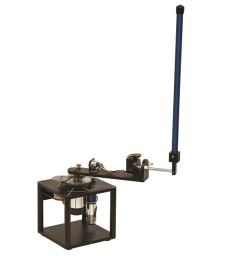
\includegraphics[width=90mm,scale=0.3]{InvertedPendulum.png}
\caption{Controlo De Pêndulo Invertido Rotativo.}\label{fig:fig2}
\end{figure}
%%%%%%%%%%%%%%%%%%%%%%%%%%%%%%%%%%%%%%%%%%%%%%%%%%%%%%%%%%%%%%%%%%%%%%%%%
%% Introdução
\newpage
 \begin{abstract} %

 
\begin{spacing}{1.5}
\indent \\ \indent O trabalho que se segue tem como objectivos fazer o projecto e análise de um sistema de controlo
em espaço de estados de um Pêndulo Invertido Rotativo \textbf{(PIR)} utilizando técnicas estocásticas. O controlo do  \textbf{PIR} apresenta um interessante desafio  dado que pelo efeito da gravidade, que actua como uma perturbação constante, a própria configuração física do pêndulo é inerentemente instável. O objetivo final do trabalho é controlar o \textbf{PIR} de maneira a manter o pêndulo na posição vertical independentemente da aplicação de possíveis perturbações aplicadas em  	\textbf{$\alpha$} alpha  ou em \textbf{$\theta$}  theta. 


Na primeira fase do trabalho foi implementado o modelo linear, que
utiliza as equações simplificadas do modelo do \textbf{PIR}, posteriormente foi implementado ainda o
modelo não linear utilizando, neste caso, as equações completas. Estas equações encontram-se descritas mais à frente neste relatório. De seguida foram projectados dois controladores, um controlador que utiliza o modelo de Ackermann e um controlador que utiliza o método \textbf{LQR} (Linear Quadratic Regulator). Ambos os controladores foram aplicados nos dois modelos (linear e não linear) nos casos de comando por tensão e de comando por binário. 

Por fim foi projectado um controlador em espaço de estados que
controla o pêndulo no ponto de equilíbrio e em simultâneo controla o braço. Foi ainda implementado e testado um controlador PID em cascata  para controlo do braço e do
pêndulo.



\end{spacing}

 \end{abstract}
\newpage
%%%%%%%%%%%%%%%%%%%%%%%%%%%%%%%%%%%%%%%%%%%%%%%%%%%%%%%%%%%%%%%%%%%%%%%%%
%% Inicio




%-------------------------------------------------------------------------
\section{Objetivos:}
O trabalho que se segue têm como objectivos fazer o projecto e análise de um sistema de controlo
em espaço de estados de um Pêndulo Invertido Rotativo (PIR) utilizando técnicas estocásticas.D
É exigido que neste projecto o pêndulo convirja sempre para a posição vertical, mesmo quando
este é sujeito a perturbações externas. É necessário projectar um controlador quadrático linear
através do uso do metodo lqr, implementar o filtro de Kalman e usá-lo como observador e ainda
projectar o filtro de Kalman com estado aumentado (estimar a perturbação).
Como objectivo principal temos a análise do PIR tanto no modelo linear como no não linear
com injecção de ruido tanto nas posições angulares como no sinal de comando e verificar como o
filtro de Kalman reage á introdução do ruido (isto é, se é capaz de filtrar os ruidos).


\begin{figure}[h]
\centering

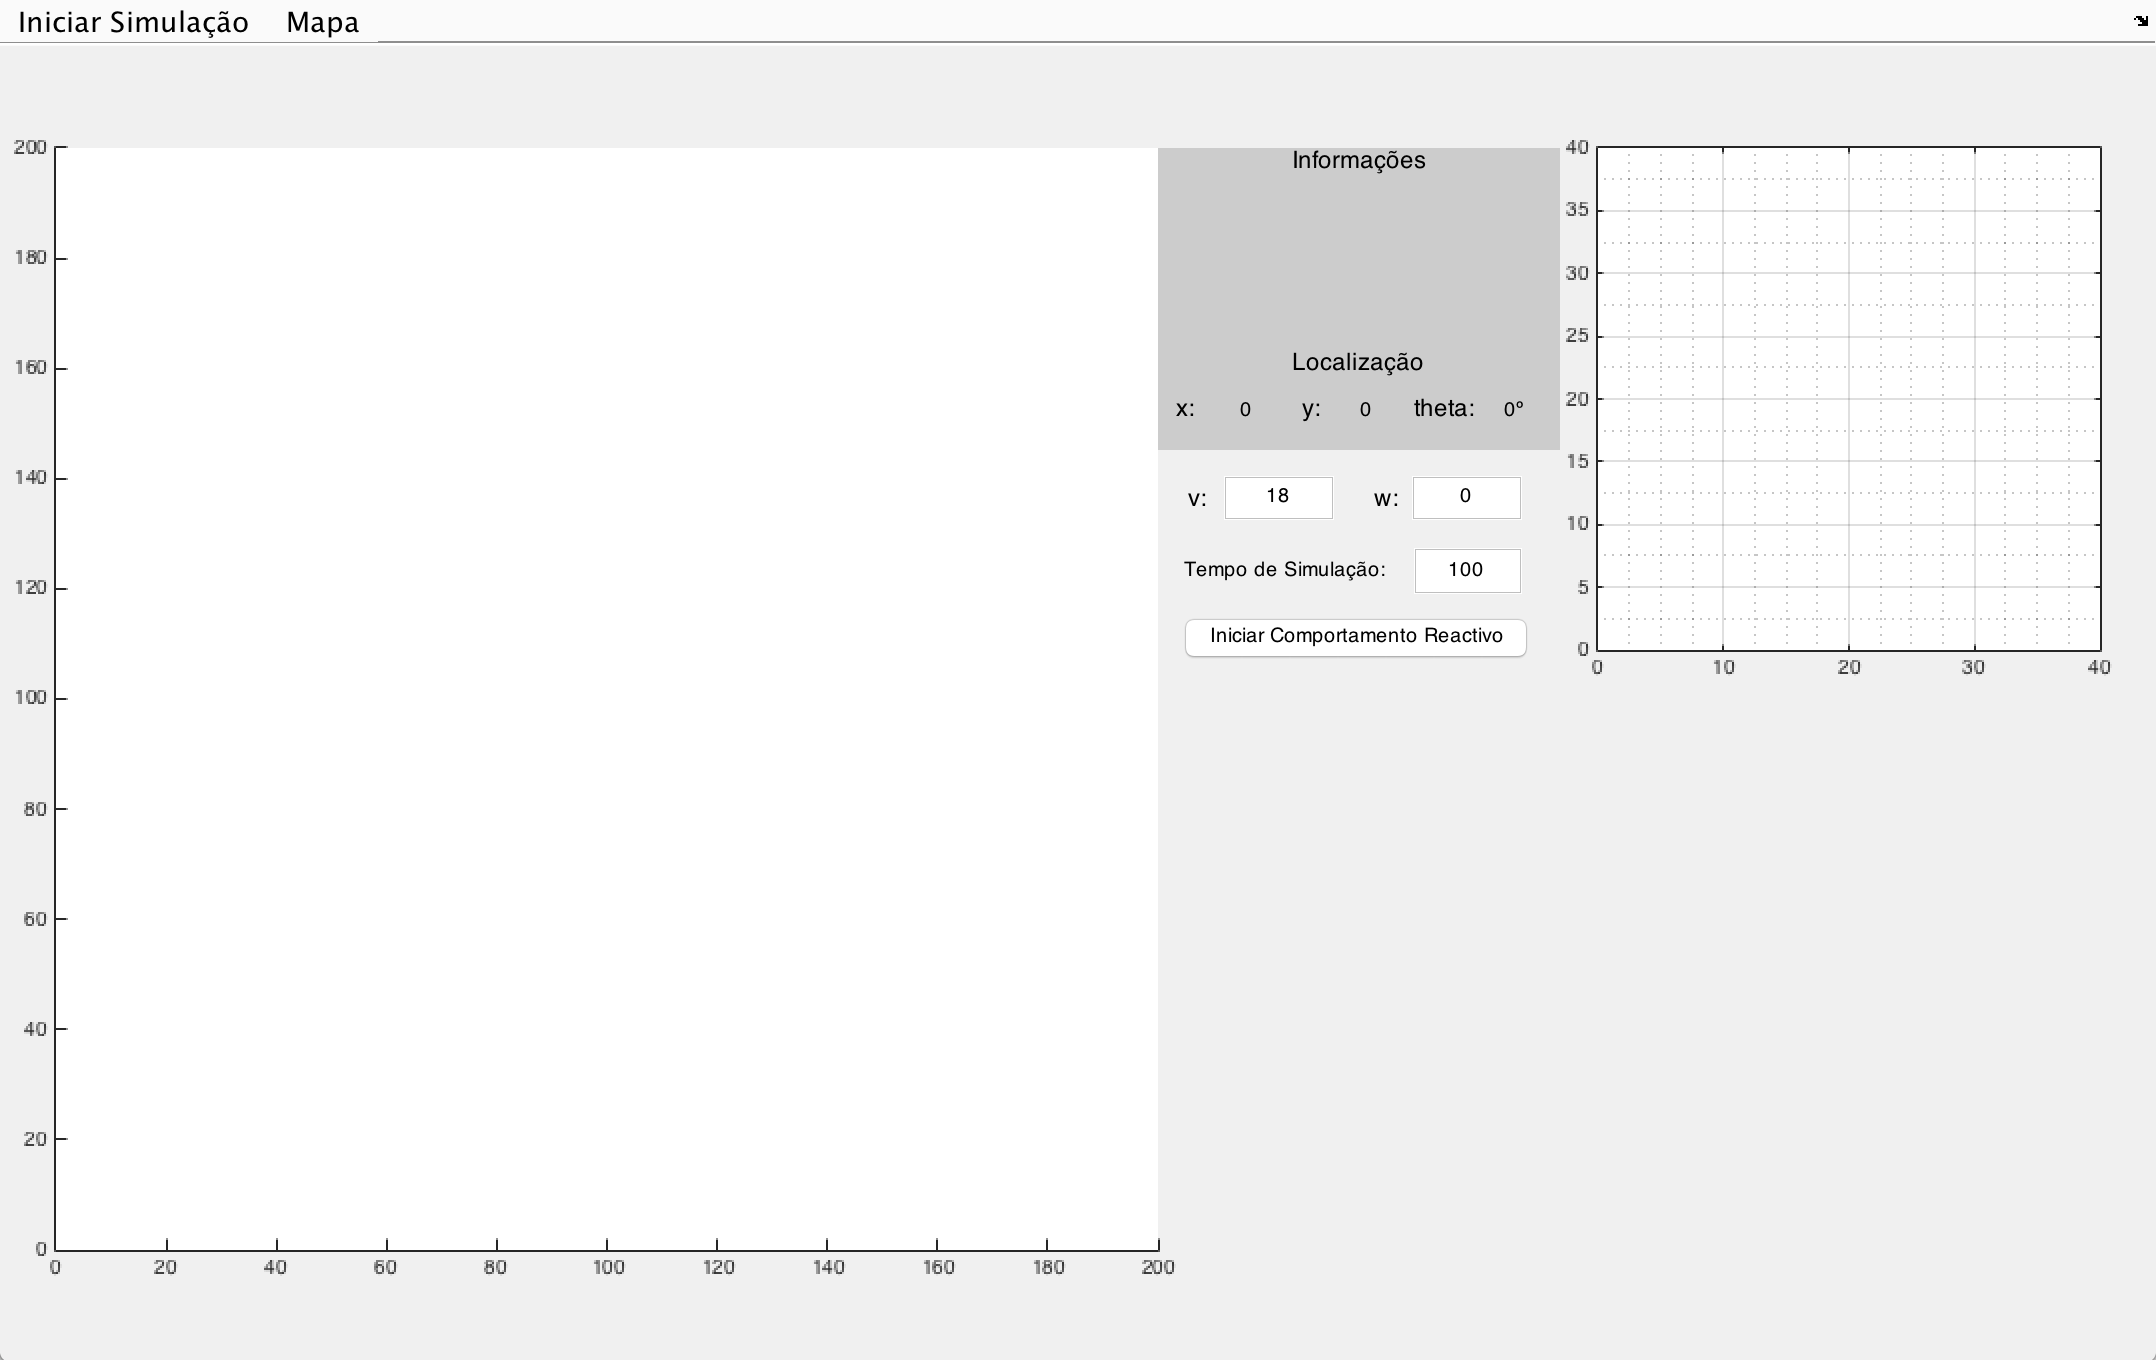
\includegraphics[width=90mm,scale=0.3]{1.png}
\caption{Captura do Simulador no momento de escolha da posição e orientação inicial. }\label{fig:fig1}
\end{figure}

\subsection{Descrição:}
Na primeira parte deste trabalho realizámos o controlo de um PIR (Pêndulo Invertido Rotativo)
usando tanto o modelo linear, como também o modelo não linear. Projectámos um controlador
usando o método LQR 1 (Regulador Quadrático Linear) fazendo uso da matriz , onde
Q 1 e Q 2 são matrizes simétricas reais definidas positivas. Os elementos da diagonal principal de
Q 1 representam o peso atribuído á posição do braço, á posição do pêndulo, á velocidade do braço
e á velocidade do pêndulo e Q 2 representa o peso atribuido ao esforço de comando do sistema. A
última matriz apenas têm um elemento visto apenas existir uma entrada no sistema.
Primeiramente foram deduzidas as fórmulas do modelo linear. Estas foram obtidas através
de um processo de linearização das equações não lineares do PIR. Após a obtenção dos dois modelos
prosseguimos para o projecto do controlador LQR, onde diferentes matrizes de Q 1 e Q 2 foram
testadas até que o sistema tivesse um bom desempenho.
Na simulação fizemos uso tanto do modelo linear como do modelo não linear e comanda-
mos o motor em tensão e em binário separadamente. De seguida fizemos uma análise cuidada da
robustez do sistema de controlo de modo a encontrar o parâmetro mais crítico. Para isso variamos
os parâmetros intrínsecos do PIR, em ambos os modelos, linear e não linear.
Na segunda parte do trabalho projectámos o filtro de Kalman e analisamos os estados esti-
mados e de seguida realimentamos o sistema com essas variáveis estimadas. Tivemos também
em consideração no projecto do observador a presença de ruído branco nas leituras de  Foi
ainda projectado um filtro de Kalman de estado aumentado quando se verifica uma perturbação
constante na entrada.
descrição resumida do trabalho com uma figura ilustrativa da
estrutura geométrica do PIR; identificar na figura as variáveis em jogo; tabela
com valores dos parâmetros do PIR.
\subsection{Principais resultados:}
descrever de forma resumida os principais
resultados observados.

\section{Modelos do Processo:}
(max 5 pags)
\subsection{Modelos lineares - casos de comando por tensão e comando por binário:}
modelos lineares do PIR, diagramas em Simulink dos sistemas de
controlo com identificação de todas as variáveis em jogo; modelos de estado c/
valores numéricos, etc...;
\subsection{Modelos não lineares - casos de comando por tensão e comando por binário:}
modelos não lineares do PIR, diagramas Simulink (esquema geral do
sistema de controlo e subsistema do modelo não linear) para os dois casos,
com identificação de todas as variáveis em jogo; código das funções MATLAB
(p/ os dois casos), etc..;
\section{Controlo em espaço de estados, aplicando a lei de Ackermann e
controlador LQR, usando na simulação os modelos linear e não linear do
PIR (max 9 pags)}
\subsection{Comando por tensão:}
- Equações dos controladores (expressões matemáticas e código em Matlab
que sintetize o núcleo do projeto); critérios e parâmetros de projecto usados;condições iniciais usadas e como foram introduzidas na implementação
MATLAB/Simulink, etc...;
- Apresentação de resultados: uma figura com apresentação sobreposta dos
sinais (ulinear, unaolinear, alfalinear, alfanaolinear) para simulação nas
mesmas condições (mesmo sinal de referência; mesmas condições iniciais;
mesmos critérios de projecto); uma figura com apresentação sobreposta dos
sinais (ulinear, unaolinear, thetalinear, thetanaolinear; discussão de
resultados (sugere-se a inclusão de uma tabela que sintetize resultados de
simulação, relativos a respostas a degrau, através do uso de indicadores como
por exemplo o tempo de pico, tempo de estabelecimento, overshoot, etc... em
função de critérios do projecto do controlador.
\subsection{Comando por binário:}
Repita os procedimentos indicados no ponto 3.1,
agora para o caso de comando por binário. Usar duas figuras/gráficos para
comparar resultados entre os dois casos em estudo (comando por tensão e
comando por binário).
Nota: comparar resultados para os dois controladores (nota: incluir
estudo/simulação para diferentes valores dos parâmetros Q e R do controlador
LQR) para as diferentes situações (comando por tensão/comando por binário;
uso do modelo linear/não linear do PIR).
\section{Controlador do pêndulo e do braço:}
(max 4 pags)
\subsection{4.1})- Faça o projeto e estudo de um controlador em espaço de estados que
realize simultaneamente o controlo do pêndulo (no ponto de equilíbrio upright)
e do braço (utilize o modelo não linear do PIR na simulação).
\subsection{4.2)}- Faça o projeto e estudo de um controlador PID em cascata (com 2 malhas
de controlo: malha interna e malha externa) para controlo do braço e do
pêndulo (no ponto de equilíbrio upright).


\section{ANEXOS} (max 6 pags)
- Anexo A: Códigos MATLAB
- Anexo B: Diagramas Simulink

% \section{References}
%\phantomsection \addcontentsline{toc}{section}{\referencesname}
%\bibliographystyle{unsrt}
%\bibliographystyle{IEEEtran}
%\bibliography{biblio}
% \nocite{*}


% \newpage
% % \thispagestyle{empty}
% \null

% \cleardoublepage
%\listoftodos




\end{document}